\title{Warm-Up for May 2nd, 2022}
\author{Dr. Jordan Hanson - Whittier College Dept. of Physics and Astronomy}
\date{\today}
\documentclass[12pt]{article}
\usepackage[a4paper, total={18cm, 27cm}]{geometry}
\usepackage{graphicx}
\usepackage{amsmath}
 
\begin{document}
\small
\maketitle
\section{Memory Bank}
\begin{enumerate}
\item Current density, and Ohm's Law: $\mathbf{J} = \rho \mathbf{v}$, $\mathbf{J} = \sigma \mathbf{E}$, $\Delta V = I R$.
\item Note about current and capacitors: $dQ/dt = I$, $Q = C\Delta V$.
\item \textit{Flux rule for motional emf}: $\mathcal{E} = - d\Phi_B/dt$
\item Definition of self-inductance, or just \textbf{inductance}: $\Phi_B = L I$.
\end{enumerate}

\section{Current and Ohm's Law}

\begin{enumerate}
\item (a) Assume that moving charges in current have two velocities: the \textit{drift velocity} $v_{\rm ave}$ in the direction of current flow, and a \textit{thermal velocity} $v_{\rm th}$ in random directions.  Let $v_{\rm th} = \lambda/t$.  Show that the average velocity of an object that is accelerating for a short time $t$ is $v_{\rm ave} = \frac{1}{2}at$. (b) Substitute $t$ with $\lambda/v_{\rm th}$, and inserve $v_{\rm ave}$ into the definition of current density from the memory bank. (c) Show that $\mathbf{J}$ is proportional to $\mathbf{E}$, even though current has a constant drift velocity $v_{\rm ave}$. \\ \vspace{1cm}
\item A capacitor $C$ has been charged up to potential $V_0$; at time $t = 0$, it is connected to a resistor $R$, and begins to discharge (Fig. \ref{fig:1}, left). (a) Determine the charge on the capacitor as a function of time, $Q(t)$.  What is the current through the resistor, $I(t)$? (b) Show that the integral of $P(t) = I^2(t)R$, the energy delivered to the resistor, is $W = \frac{1}{2}CV_0^2$. (c) Now imagine charging up the capacitor (Fig. \ref{fig:1}, middle).  Determine $Q(t)$ and $I(t)$. (d) Find the total energy output of the battery ($\int V_0 I dt$).  What fraction of the battery output shows up in the capacitor? \\ \vspace{2cm}
\item For the RL circuit of Fig. \ref{fig:1} (right), what is $I(t)$?
\end{enumerate}

\begin{figure}
\centering
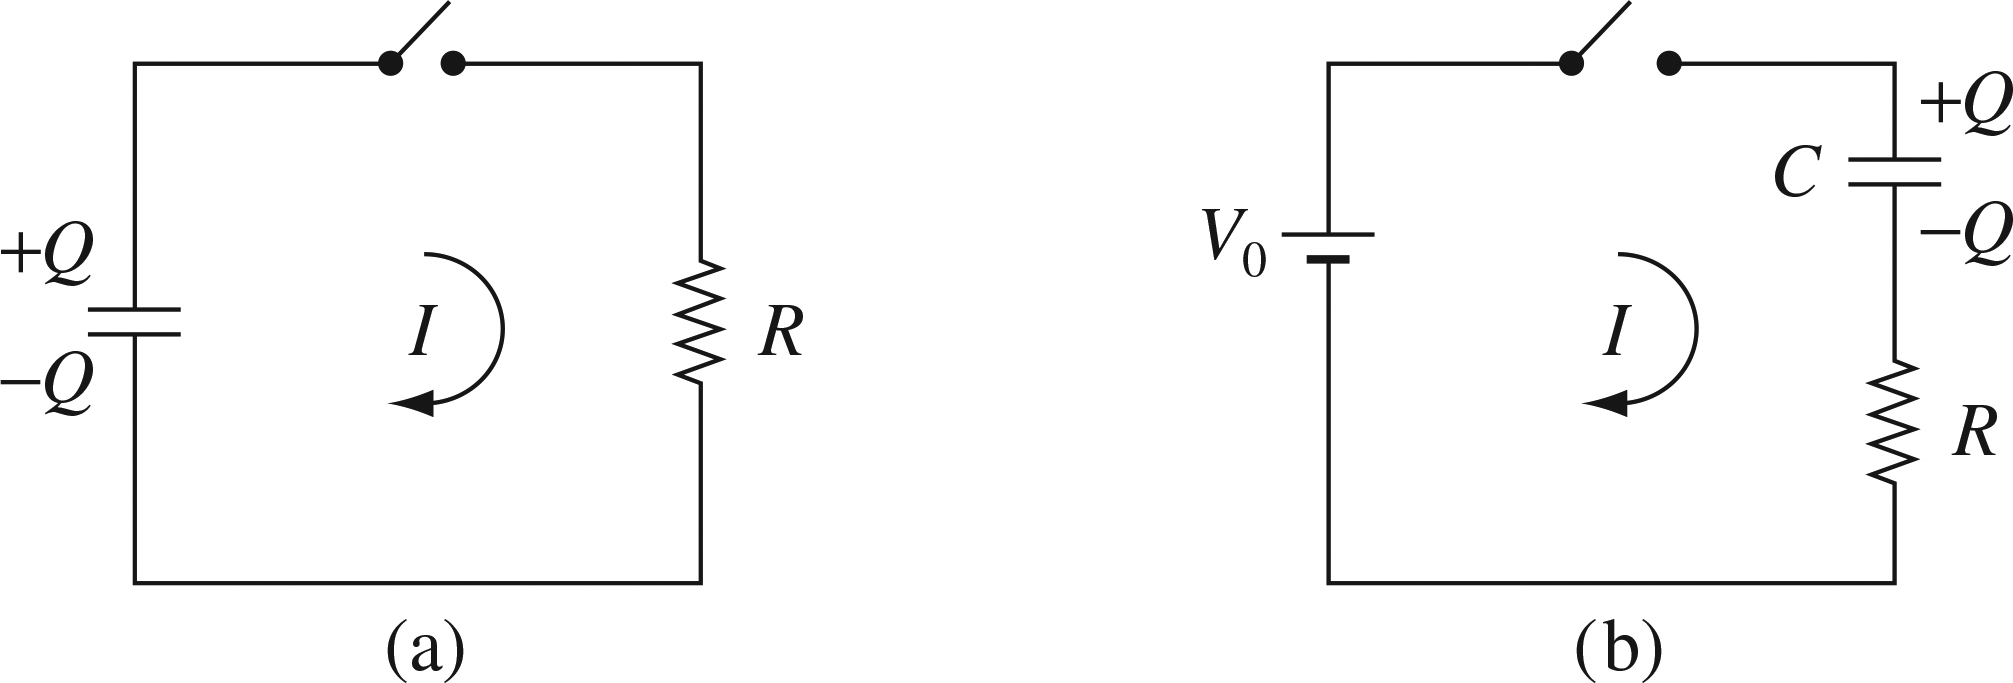
\includegraphics[width=0.5\textwidth]{figures/7_5.jpg} \hspace{1cm}
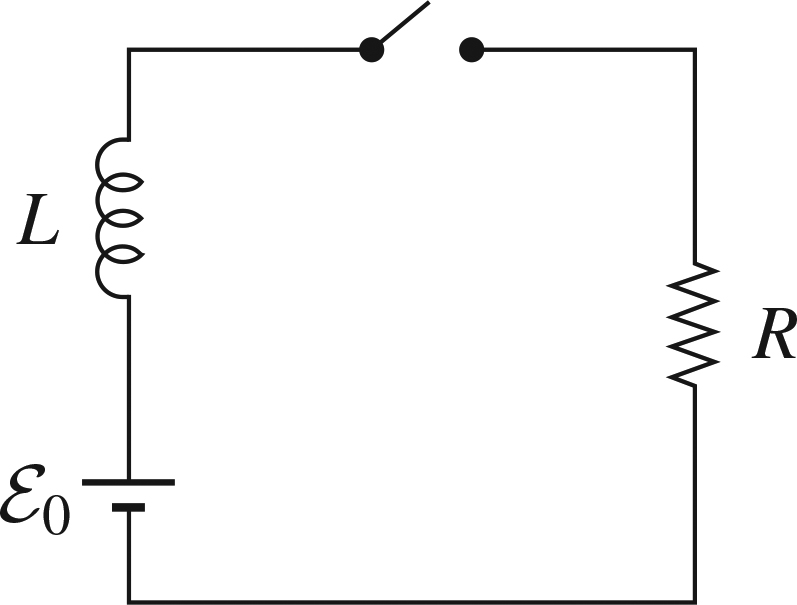
\includegraphics[width=0.25\textwidth]{figures/7_35.jpg}
\caption{\label{fig:1} Two circuits: (left) RC circuits, and (right) the RL circuit.}
\end{figure}

\end{document}